% !TeX TS-program = pdflatex
% !TeX encoding = UTF-8
% !TeX spellcheck = nl_NL



%% Warn me about obsolete Latex stuff
\RequirePackage[l2tabu, orthodox]{nag}

%% Some credentials about the author
\newcommand{\bookauthor}{Jesse op den Brouw}
\newcommand{\booktitleI}{ATmega32}
\newcommand{\booktitleII}{}
\newcommand{\booktitle}{\booktitleI{} \booktitleII}
\newcommand{\booksubtitle}{software-ontwikkeling in\\ assembler en C}
\newcommand{\bookinstitution}{De Haagse Hogeschool}
\newcommand{\bookedition}{Eerste druk}
\newcommand{\bookversion}{0.1}
\newcommand{\bookkeywords}{AVR ATmega32 hardware software microcontroller assembler}
\newcommand{\email}{J.E.J.opdenBrouw@hhs.nl}
%% Nice text on empty pages, or not...
\newcommand{\thispageintentionallyleftblank}{Deze pagina is opzettelijk leeg gelaten.}
%\newcommand{\thispageintentionallyleftblank}{}
\newcommand{\bookuseadvanded}{\useadvancedfalse}
%% Pick one or none, placed in outer upper corner
\newcommand{\finalconceptdraft}{CONCEPT}

\newcommand{\bookpartI}{\usebookpartIfalse}
\newcommand{\bookpartII}{\usebookpartIItrue}
\newcommand{\bookpartIII}{\usebookpartIIIfalse}
\newcommand{\bookasbook}{\usebookasbookfalse}



%%%%%%%%%%%%%%%%%%%%%%%%%%%%%%%%%%%%%%%%%%%%%%%%%%%%%%%%%%%%%%%%%%
%%%
%%%       PREAMBLE
%%%
%%%%%%%%%%%%%%%%%%%%%%%%%%%%%%%%%%%%%%%%%%%%%%%%%%%%%%%%%%%%%%%%%%

%% 12pt charachters, A4 paper size, twoside printing, equation left aligned
%% equation indent at 1 em
\documentclass[12pt,a4paper,final,twoside,fleqn]{book}

% Set widow penalty
\clubpenalty2000

%% Use T1 output font encoding
\usepackage[T1]{fontenc}

%% Copy credentials
\renewcommand{\author}{\bookauthor}
\renewcommand{\title}{\booktitle}
\renewcommand{\date}{\today}

%% Some defines for scaling figs
%% Scaled 1/1
\def\figscale{0.6} % Really it should be 1-exp{-1} = 0.63212055882855767840447622983854
\def\figscaleA{0.5}
\def\figscaleAA{0.43}
\def\figscaleB{0.3}
\def\figscaleC{1.0}
\def\figscaleE{0.7}
\def\figscaleF{0.6}
\def\figscaleG{0.8}

%% Define which part of the book is included
\newif\ifusebookpartI\bookpartI
\newif\ifusebookpartII\bookpartII
\newif\ifusebookpartIII\bookpartIII
\newif\ifusebookasbook\bookasbook

%% Dutch spelling of chapter, section, etc.
\usepackage[dutch]{babel}
%% Set American style quotes
\usepackage[style=american]{csquotes}

%% Set page layout
\usepackage[a4paper,bindingoffset=0.2in,left=1.0in,right=1.0in,top=1.0in,bottom=1.4in,
                                                               footskip=0.5in]{geometry}
                                                               
%% Use of dashed lines in tables
\usepackage{tabu}
\usepackage{tabularx}
\usepackage{booktabs}
\usepackage{multirow}

%% Use array's
\usepackage{array}

%% Define and use colors
\usepackage[x11names,table]{xcolor}

%% Include rotating (includes graphicx) packages
\usepackage{rotating}

%% Nice calculations with lengths
%% Note: calc has to be loaded before enumitem
\usepackage{calc}

%% Enumerate items
\usepackage[inline]{enumitem}
%% Use an asterisk before item number, see
%% http://tex.stackexchange.com/questions/61263/add-an-asterisk-left-of-an-enumerate
\setlist[enumerate]{before=\setupmodenumerate}
%
\newif\ifmoditem
\newcommand{\setupmodenumerate}{%
  \global\moditemfalse
  \let\origmakelabel\makelabel
  \def\moditem##1{\global\moditemtrue\def\mesymbol{##1}\item}%
  \def\makelabel##1{%
%    \origmakelabel{\ifmoditem\llap{\mesymbol\enspace}\fi##1}%
    \origmakelabel{\ifmoditem\llap{\mesymbol\ }\fi##1}%
    \global\moditemfalse}%
}
\newcommand{\itemstar}{\moditem{\textbf{*}}}

%% Use floats
\usepackage{float}
%% Separation between floats 12pt --> 24 pt
\setlength{\floatsep}{24.0pt plus 2.0pt minus 2.0pt}

%% Using footnotes in tables
%%%\usepackage{tablefootnote}
\usepackage{threeparttable}
%\renewcommand{\TPTminimum}{1em}
\renewcommand{\TPTnoteSettings}{\footnotesize}
%\makeatletter
%\setlist[tablenotes]{label=\tnote{\alph*},ref=\alph*,itemsep=\z@,topsep=\z@skip,partopsep=\z@skip,parsep=\z@,itemindent=\z@,labelindent=\tabcolsep,labelsep=.2em,leftmargin=*,align=left,before={\footnotesize}}
%\makeatother

% http://archive.cs.uu.nl/mirror/CTAN/macros/latex/contrib/biblatex/doc/biblatex.pdf
\PassOptionsToPackage{hyphens}{url}
\usepackage[
    backend=biber,
    backref=true,
    backrefstyle=none,
    sortcites=true,
    sorting=none,
    doi=false, % doi informatie wordt niet weergegeven
    %uniquename=true,
    %uniquelist=true,
    maxcitenames=3,
    %issn=false, werkt niet
    language=american
]{biblatex}
\addbibresource{book_citations.bib}
\DefineBibliographyStrings{dutch}{
    backrefpage = {blz.},
    backrefpages = {blz.},
}
%% Do not show ISSN numbers
\AtEveryBibitem{\clearfield{issn}}
\AtEveryCitekey{\clearfield{issn}}

%% Use the AMS Mathematical characters, no other AMS packages required
\usepackage{mathtools}
\usepackage{siunitx}
\sisetup{output-decimal-marker = {,}}
\sisetup{tophrase={{\ en\ }}}
%\usepackage{amssymb}
\setlength{\mathindent}{1em}
\DeclareMathSymbol{,}{\mathord}{letters}{"3B}
\abovedisplayskip=30pt
\belowdisplayskip=30pt
\abovedisplayshortskip=30pt
\belowdisplayskip=30pt

%% Find out what engine we're running...
\usepackage{ifluatex,ifxetex}

%% Settings for fonts et al.
\ifnum 0\ifxetex 1\fi\ifluatex 1\fi>0
\usepackage[math-style=TeX]{unicode-math}
%\usepackage{unicode-math}
\usepackage{fontspec}
\setmainfont[Ligatures=TeX]{Calibri}
\defaultfontfeatures{Scale=MatchUppercase}
\setsansfont{Calibri}
\setmonofont{Consolas}
\setmathfont[slash-delimiter=frac]{Cambria Math}
\setmathfont[range=up]{Calibri}
\setmathfont[range=it]{Calibri Italic}
\setmathfont[range=bfup]{Calibri Bold}
\setmathfont[range=bfit]{Calibri Bold Italic}
\setoperatorfont\normalfont % For log, sin, cos, etc.
\def\checkmark{\textsl{v}}
\def\muup{μ}
\makeatletter
\DeclareRobustCommand{\LaTeX}{L\kern-.20em%
        {\sbox\z@ T%
         \vbox to\ht\z@{\hbox{\check@mathfonts
                              \fontsize\sf@size\z@
                              \math@fontsfalse\selectfont
                              A}%
                        \vss}%
        }%
        \kern-.06em%
        \TeX}
\makeatother
\else
%% Use the Charter and Nimbus Mono fonts
\usepackage{nimbusmono}
%\usepackage{charter}
\usepackage[bitstream-charter]{mathdesign}
%% Use microtype
\usepackage[stretch=10]{microtype}
\pdfminorversion=5
\pdfobjcompresslevel=1
%% Set input encoding to UTF-8
\usepackage[utf8]{inputenc}
\makeatletter
\DeclareRobustCommand{\LaTeX}{L\kern-.20em%
        {\sbox\z@ T%
         \vbox to\ht\z@{\hbox{\check@mathfonts
                              \fontsize\sf@size\z@
                              \math@fontsfalse\selectfont
                              A}%
                        \vss}%
        }%
        \kern-.05em%
        \TeX}
\makeatother
\fi

%%
%% Find out which engine is running
\newcount\bookmajorversion
\newcount\bookminorversion

\ifluatex
\bookmajorversion=\luatexversion
\bookminorversion=\luatexversion
\divide \bookmajorversion by 100
\multiply \bookmajorversion by 100
\advance \bookminorversion by -\bookmajorversion
\divide \bookmajorversion by 100
\def\booktexbanner{Lua\LaTeX\ \the\bookmajorversion.\the\bookminorversion.\luatexrevision}
\else
\ifxetex
\bookmajorversion=\XeTeXversion
\def\booktexbanner{Xe\LaTeX\ \the\bookmajorversion\XeTeXrevision}
\else
\bookmajorversion=\pdftexversion
\bookminorversion=\pdftexversion
\divide \bookmajorversion by 100
\multiply \bookmajorversion by 100
\advance \bookminorversion by -\bookmajorversion
\divide \bookmajorversion by 100
\def\booktexbanner{pdf\LaTeX\ \the\bookmajorversion.\the\bookminorversion.\pdftexrevision}
\fi
\fi

%%
%% Do we include advanced sections?
\newif\ifuseadvanced\bookuseadvanded

%%
%% Creating advanced sections with * prepended to sec number
\newcommand*{\secmark}{}
\newcommand*{\marktotoc}[1]{\renewcommand{\secmark}{#1}}
\newcommand*{\advanced}{%
  \renewcommand*{\secmark}{*}%
  \addtocontents{toc}{\protect\marktotoc{*}}%
}
\newcommand*{\basic}{%
  \renewcommand*{\secmark}{}%
  \addtocontents{toc}{\protect\marktotoc{}}%
}

% http://archive.cs.uu.nl/mirror/CTAN/macros/latex/contrib/titlesec/titlesec.pdf
\usepackage{titlesec}
\usepackage{titletoc}
\usepackage[titles]{tocloft}
\newcommand{\chapnumfont}{%     % define font for chapter number
  \usefont{T1}{pnc}{b}{n}%      % choose New Chancery, bold, normal shape
  \fontsize{100}{100}%          % font size 100pt, baselineskip 100pt
  \selectfont%                  % activate font
  \vspace*{-0.5\baselineskip}	% half baseline skip up
}
\titleformat{\chapter}[display]
{\bfseries}
{\chapnumfont\color{chapnumcolor}{\thechapter}}
{0ex}
{\ifnum 0\ifxetex 1\fi\ifluatex 1\fi>0\else\fontfamily{phv}\selectfont\fi\Huge\bfseries}
[{\vspace*{1ex}\titlerule[0.8pt]}]
\titleformat{\section}{\ifnum 0\ifxetex 1\fi\ifluatex 1\fi>0\else\fontfamily{phv}\selectfont\fi\large\bfseries}{\secmark\thesection}{1em}{}
\titleformat{\subsection}{\ifnum 0\ifxetex 1\fi\ifluatex 1\fi>0\else\fontfamily{phv}\selectfont\fi\bfseries}{\secmark\thesubsection}{1em}{}
\titlespacing*{\section}{0pt}{\baselineskip}{0.4\aftersubsection}
\titlespacing*{\subsection}{0pt}{.8\baselineskip}{0.0\aftersubsection}
\titlespacing*{\subsubsection}{0pt}{.6\baselineskip}{0pt}
\titlespacing*{\paragraph}{0pt}{1.0ex plus 1ex minus .2ex}{1.5em}
\newlength{\aftersubtitle}
\setlength{\aftersubtitle}{1.2\baselineskip}
\newlength{\aftersubsection}
\setlength{\aftersubsection}{\aftersubtitle}
\addtolength{\aftersubsection}{-\baselineskip}
\titlespacing*{\subsection}{0pt}{.8\baselineskip}{\aftersubsection}
\titlespacing*{\subsubsection}{0pt}{.6\baselineskip}{0pt}
%\titlecontents{section}[1.5em]{}{\contentslabel[\secmark\thecontentslabel]{1.5em}}{}{\titlerule*{}\bfseries\contentspage}
%\titleformat{\section}{\normalfont\Large\bfseries}{\makebox[1.5em][l]{\secmark\thesection}}{0.4em}{}
%\titlecontents{section}[1.5em]{}{\bfseries\contentslabel[\secmark\thecontentslabel]{1.5em}}{\hspace*{-1.5em}}{\titlerule*{}\bfseries\contentspage}
%\usepackage{tocloft,etoolbox}
%\makeatletter
%\patchcmd{\l@section}{#1}{\settowidth{\mylength}{\secmark}\hspace*{-\mylength}\secmark{#1}}{}{}
%\renewcommand\cftchappresnum{\chaptername\newline}
%\setlength{\cftchapnumwidth}{3.5cm}
%\renewcommand{\cfttoctitlefont}{\fontfamily{phv}\selectfont\Huge\bfseries\scshape}
%\renewcommand{\cftaftertoctitle}{}
%\setlength{\cftbeforetoctitleskip}{\baselineskip}
%\setlength{\cftaftertoctitleskip}{\aftersubsection}
%% Remove page number on first page of ToC
\AtBeginDocument{\addtocontents{toc}{\protect\thispagestyle{fancy}}}
%% Make space for page number in TOC wider
\makeatletter
\renewcommand\@pnumwidth{1cm}
\makeatother
%% Wider chapnum and secnum
%\renewcommand*\cftchapnumwidth{2em}
\renewcommand*\cftsecnumwidth{3em}

% http://archive.cs.uu.nl/mirror/CTAN/macros/latex/contrib/footmisc/footmisc.pdf
% ruimte onder aan de pagina tussen tekst en voetnoot niet na voetnoot
% package moet VOOR fancyhdr om warning te voorkomen
\usepackage[
    bottom,
    hang,
    multiple
]{footmisc}
% inspringen
\setlength{\footnotemargin}{1em}
% ruimte tussen footnotes:
\setlength{\footnotesep}{.6\baselineskip}


%% Using fancy headers and footers
%% http://ftp.snt.utwente.nl/pub/software/tex/macros/latex/contrib/fancyhdr/fancyhdr.pdf
\usepackage{fancyhdr}
\newcommand{\bookfancy}{
    \fancyhead{} % clear all header fields
    \fancyhead[LE,RO]{\footnotesize\finalconceptdraft}
    %\fancyhead[RO,LE]{\thepage} % Right Odd, Left Even
    \fancyfoot{} % clear all footer fields
    \fancyfoot[LE,RO]{\thepage}   % page number in "outer" position of footer line
    \fancyfoot[RE,LO]{\booktitle} % other info in "inner" position of footer line
    \renewcommand{\headrulewidth}{0pt}
    \renewcommand{\footrulewidth}{0.4pt}
}
\pagestyle{fancy}
\bookfancy
\fancypagestyle{plain}{\bookfancy}
%% Clear header and footer for blank pages, possibly print "This page ..."
\makeatletter
\renewcommand*{\cleardoublepage}{\clearpage\if@twoside \ifodd\c@page\else
\hbox{}\vfill\begin{center}\thispageintentionallyleftblank\end{center}\vfill\vfill%
\thispagestyle{empty}%
\newpage%
\if@twocolumn\hbox{}\newpage\fi\fi\fi}
\makeatother

%% Indexing words...
\usepackage[noautomatic]{imakeidx}
%% The index page is typeset...
\indexsetup{othercode=\footnotesize\thispagestyle{fancy}}
\makeindex[columns=2]
%\usepackage{showidx}

%% Making captions nicer...
\usepackage[font=footnotesize,format=plain,labelfont=bf,up,textfont=sl,up]{caption}
\DeclareCaptionLabelSeparator{emdash}{\ \ ---\ \ }
\usepackage[labelformat=simple,font=footnotesize,format=plain,labelfont=bf,textfont=sl]{subcaption}
\captionsetup[figure]{format=hang,justification=centering,singlelinecheck=off,skip=2ex}
\captionsetup[table]{format=hang,justification=centering,singlelinecheck=off,skip=2ex}
\captionsetup[subfigure]{format=hang,justification=centering,singlelinecheck=off,skip=2ex}
\captionsetup[subtable]{format=hang,justification=centering,singlelinecheck=off,skip=2ex}
%% Put parens around the subfig name (a) (b) etc. Needs labelformat simple
\renewcommand\thesubfigure{(\alph{subfigure})}
\renewcommand\thesubtable{(\alph{subtable})}

% Parskip et al.
\usepackage{parskip}[=v1]
\makeatletter
\setlength{\parfillskip}{00\p@ \@plus 1fil}
\makeatother

%% Nice strike out of text (more used in numbers)
\usepackage{cancel}

%% Some colors
\definecolor{dkgreen}{rgb}{0,0.6,0}
%\definecolor{gray}{rgb}{0.5,0.5,0.5}
\definecolor{mauve}{rgb}{0.58,0,0.82}
%\definecolor{lightgray}{rgb}{0.95,0.95,0.95}
\definecolor{GKYgray}{rgb}{0.65,0.65,0.65}
\definecolor{lightpink}{HTML}{F8E0E0}%{FBF3F3}%
\definecolor{thuasgreen}{RGB}{158,167,0}
\definecolor{thuasgreen2}{RGB}{159,169,89}
\ifusebookasbook
\colorlet{bookcolor}{black}
\colorlet{chapnumcolor}{gray!90}
\colorlet{listingnumbercolor}{bookcolor}
\colorlet{listingbgcolor}{gray!10}
\colorlet{infoboxbg}{gray!5}
\colorlet{infoboxbgtitle}{gray!15}
\colorlet{venndiagramcolor}{lightgray}
\colorlet{regcell}{gray!90}
\else
\colorlet{bookcolor}{thuasgreen!50!black}
\colorlet{chapnumcolor}{thuasgreen}
\colorlet{listingnumbercolor}{thuasgreen!50!black}
\colorlet{listingbgcolor}{thuasgreen!50!white}
%\colorlet{listingcolor}{SkyBlue2!30!white}
\colorlet{infoboxbg}{blue!5}
\colorlet{infoboxbgtitle}{blue!15}
\colorlet{venndiagramcolor}{blue!15}
\colorlet{regcell}{thuasgreen!50!white}
\fi

%% Use computer code listings
\usepackage{listings}
%% Use textcomp for upright quotes in listings
\usepackage{textcomp}

%% Define listing style for VHDL
\lstset{%
  language=VHDL,
  basicstyle=\footnotesize\ttfamily,
  numbers=left,
  numberstyle=\tiny\color{listingnumbercolor},
  stepnumber=1,                           
  numbersep=8pt,
  backgroundcolor=\color{listingbgcolor},
  showspaces=false,
  showstringspaces=false,
  showtabs=false,
  frame=lines,
  rulecolor=\color{bookcolor},
  tabsize=4,
  captionpos=b,
  breaklines=true,
  breakatwhitespace=false,
  title=\lstname,
  upquote=true,
  aboveskip=\baselineskip
}

%% Using hyperrefs...
\usepackage{hyperref}
\ifusebookasbook
\hypersetup{
	colorlinks=true,
	linkcolor=black,
	citecolor=black,
	urlcolor=black,
    pdftitle={\booktitleI\ \booktitleII, \booksubtitle},
    pdfauthor={\bookauthor},
    %pdfsubject={Beginselen van de digitale techniek},
    pdfsubject={},
    pdfkeywords={\bookkeywords},
	pdfdisplaydoctitle=true,
	pdfpagelayout=TwoPageRight
}
\else
\hypersetup{
	colorlinks=true,
	linkcolor=bookcolor,
	citecolor=bookcolor,
	urlcolor=bookcolor,
    pdftitle={\booktitleI\ \booktitleII, \booksubtitle},
    pdfauthor={\bookauthor},
    %pdfsubject={Beginselen van de digitale techniek},
    pdfsubject={},
    pdfkeywords={\bookkeywords},
	pdfdisplaydoctitle=true,
	pdfpagelayout=TwoPageRight
}
\fi
\urlstyle{sf}%

%% Lay things over a picture
%% http://mirrors.ctan.org/macros/latex/contrib/overpic/opic-abs.pdf
\usepackage[abs]{overpic}

%% Set \FloatBarrier to empty
\def\FloatBarrier{}

%% Create EAN13 ISBN number figure
\usepackage{ean13isbn}

%%%
%%% LaTeX installed packages loading done here
%%%
%%% From here on, only own-written packages and commands
%%%

%% Better overline command for use in logic functions
\newcommand*{\oline}[1]{\overline{#1\mathstrut}}

%% A nice circled x for use in prime implicant tables
\newcommand{\cx}{\raisebox{-1.2pt}{\textcircled{\raisebox{1.2pt}{x}}}}

%% Prints nice "solution" header (dutch: uitwerking)
\newcommand{\uitw}[1]{\addvspace{1em}\textbf{Uitwerking opgave \ref{#1}.}\vspace*{0.2em}\newline}

%% Circled numbers
%\def\circled#1{{\ooalign{\hfil\lower.1ex\hbox{#1}\hfil\crcr\Orb}}}
\def\circled#1{\textcircled{\raisebox{.95pt}{\scriptsize #1}}}

%% Typeset propositions and postulates
\newcommand{\propositie}[1]{\par\hspace*{1em}#1\par}

%% Log notation with base
\newcommand\logbase[1]{\mathop{{}^{#1}\mathrm{log}}}

%% To input and print files.
%% \booklising{lang}{caption}{filename}{ext}{floatplace}
%%%\newcommand{\booklisting}[5]{%
%%%\begin{figure}[#5]%
%%%\lstinputlisting[language=#1,caption={#2.},label=cod:#3]{code/#3.#4}%
%%%\vspace*{-\baselineskip}
%%%\end{figure}%
%%%}
\newcommand{\booklisting}[6][]{%
\begin{figure}[#6]%
\lstinputlisting[language=#2,caption={#3.},label=cod:#4,#1]{code/#4.#5}%
\vspace*{-\baselineskip}
\end{figure}%
}
%\lstinputlisting[language=#1,caption={#2.},label=cod:#3,float]{code/#3.vhd}%
%\lstinputlisting[language=#1,caption={#2.},label=cod:#3,float,floatplacement=h]{code/#3.vhd}%
%\begin{minipage}{\textwidth}%
%\lstinputlisting[language=#1,caption={#2.},label=cod:#3]{code/#3.vhd}%
%\end{minipage}%
%%% werkt niet
%%%\captionsetup{belowskip=100pt}
%%%\setlength{\abovecaptionskip}{-100pt plus 0pt minus 0pt}

\newcommand{\lstmodelsim}[1]{\lstinline[language=modelsim]|#1|}   %[
\newcommand{\lstvhdl}[1]{\lstinline[language=vhdl]|#1|}   %[
\newcommand{\lstc}[1]{\lstinline[language=C]|#1|}   %[
\newcommand{\lstpseu}[1]{\lstinline[language=HHSEprocPseudoLang]|#1|}   %[
\newcommand{\lstasm}[1]{\lstinline[language=HHSEprocAssembler]|#1|}   %[

%% To put single figures
%% \bookfigure{floatplace}{scale}{imagename}{caption}{label}
\newcommand{\bookfigure}[5]{%
\begin{figure}[#1]%
\centering%
\includegraphics[scale=#2]{images/#3}%
\caption{#4.}%
\label{fig:#5}%
\end{figure}%
}

%% Print hidden characters by using the white color, used for aligning numbers.
%% Please note that the dash must cast to mathbin. See:
%% http://tex.stackexchange.com/questions/21598/how-to-color-math-symbols
\newcommand\ph[1]{\if-#1\mathbin{\textcolor{white}{-}}\else\textcolor{white}{#1}\fi}

%% Lesser and more space around the binay dot and plus and xor
\let\oldcdot\cdot
\renewcommand{\cdot}{\kern-.10em\oldcdot\kern-.10em}
\newcommand{\cdotw}{\kern.08em\oldcdot\kern.08em}
\newcommand{\cdotww}{\kern.16em\oldcdot\kern.16em}
\newcommand{\plusw}{\kern.08em+\kern.08em}
\newcommand{\plusww}{\kern.16em+\kern.16em}
\newcommand{\oplusw}{\kern.08em\oplus\kern.08em}
\newcommand{\oplusww}{\kern.16em\oplus\kern.16em}

%% Vertically align cell contents
\newcolumntype{M}[1]{>{\centering\arraybackslash$\vcenter\bgroup\hbox\bgroup}m{#1}<{\egroup\egroup$}}
\newcolumntype{C}{>{\centering\arraybackslash$\vcenter\bgroup\hbox\bgroup}c<{\egroup\egroup$}}

%% Make cells in tables vertically wider
\newcommand\Tstrut{\rule{0pt}{2.0ex}}         % = `top' strut
\newcommand\Bstrut{\rule[-0.9ex]{0pt}{0pt}}   % = `bottom' strut

%% Check if a label exists
\makeatletter
\newcommand{\iflabelexists}[3]{\@ifundefined{r@#1}{#3}{#2}}
\makeatother

%% Using tcolorbox for Infobox environment settings
\usepackage[most]{tcolorbox}
\newtcolorbox{infobox}[1][]{title=#1,colback=infoboxbg,colframe=bookcolor,fonttitle=\large\scshape,colbacktitle=infoboxbgtitle,coltitle=black,toptitle=5pt,bottomtitle=5pt,sharp corners,boxrule=2pt,titlerule=0pt,top=7pt,parbox=false,floatplacement=!b,float=!b}

\newcounter{example}[chapter]
\setcounter{example}{0}
\newtcolorbox[use counter=example,number within=chapter,list inside=example]{example}[1][]{%
    % Example Frame Start
    empty,% Empty previously set parameters
    title={Voorbeeld \theexample\ifx\hfuzz#1\hfuzz \else : #1\fi},% use \thetcbcounter to access the example counter text
%	list entry=Voorbeeld~\theexample.\quad#1,
    % Attaching a box requires an overlay
    attach boxed title to top left,
    % Ensures proper line breaking in longer titles
    minipage boxed title,
    % (boxed title style requires an overlay)
    boxed title style={empty,size=minimal,toprule=0pt,top=4pt,bottom=2pt,left=3mm,overlay={}},
    coltitle=bookcolor,fonttitle=\bfseries,
    before=\par\medskip\noindent,parbox=false,boxsep=0pt,left=3mm,right=0mm,top=5pt,breakable,pad at break=0mm,
       before upper=\csname @totalleftmargin\endcsname0pt, % Use instead of parbox=true. This ensures parskip is inherited by box.
    % Handles box when it exists on one page only
    overlay unbroken={\draw[bookcolor,line width=.5pt] ([xshift=-0pt]title.north west) -- ([xshift=-0pt]frame.south west); },
    % Handles multipage box: first page
    overlay first={\draw[bookcolor,line width=.5pt] ([xshift=-0pt]title.north west) -- ([xshift=-0pt]frame.south west); },
    % Handles multipage box: middle page
    overlay middle={\draw[bookcolor,line width=.5pt] ([xshift=-0pt]frame.north west) -- ([xshift=-0pt]frame.south west); },
    % Handles multipage box: last page
    overlay last={\draw[bookcolor,line width=.5pt] ([xshift=-0pt]frame.north west) -- ([xshift=-0pt]frame.south west); },%
}
\makeatletter % no indent for entries
\renewcommand{\l@tcolorbox}{\@dottedtocline{1}{0pt}{2.3em}}
\makeatother

%% Hypenation of some uncommon words in Dutch
\hyphenation{Kar-naugh-dia-gram Kar-naugh-dia-gram-men min-term min-ter-men flip-flop flip-flops im-pli-cant im-pli-can-ten twee-tal-len vier-tal-len acht-tal-len zes-tien-tal-len timing-dia-gram-men timing-dia-gram toe-stands-dia-gram toe-stands-dia-grammen ge-schre-ven}

%% The really backmatter
\newcommand{\bookbackmatter}{%
\ifusebookasbook
\cleardoublepage%
\hspace*{0pt}
\thispagestyle{empty}
\clearpage
\pagecolor{SkyBlue2}
\hspace*{0pt}
\vfill
%\hfill\EANisbn[SC5b,ISBN=978-80-7340-097-2] 
\thispagestyle{empty}
\fi
}

%%% No package loading from here

\newcolumntype{Y}{>{\centering\arraybackslash}X}
%\newcolumntype{Y}{X}

\usepackage{tikz}
%\usetikzlibrary{arrows}
\usepackage{marvosym}
%\usepackage{graphicx}

\usepackage{longtable}

\newenvironment{registerdef}[3][!ht]{
\edef\regdefa{#2}
\edef\regdefb{#3}
\figure[#1]
\renewcommand\arraystretch{1.4}
\scriptsize
\centering
\tabularx{0.9\textwidth}{YYYYYYYY}
}{
\endtabularx
\caption{\regdefa.}
\label{\regdefb}
\endfigure
}

\lstdefinelanguage{AVRassembler}{
morekeywords=[1]{adc,add,adiw,andi,asr,bclr,bld,brbc,brbs,brcc,brcs,break,breq,brge,brhc,brhs,brid,brie,brlo,brlt,brmi,brne,brpl,brsh,brtc,brts,brvc,brvs,bset,bst,cbi,cbr,clc,clh,cli,cln,clr,cls,clt,clv,clz,com,count,cp,cpc,cpi,cpse,dec,eicall,eijmp,elpm,end,eor,espm,fmul,fmuls,fmulsu,in,inc,ld,ldd,ldi,lds,lsl,lsr,mov,movw,neg,nop,ori,out,pop,push,rcall,ret,reti,rjmp,rol,sbc,sbci,sbi,sbic,sbis,sbiw,sbr,sbrc,sbrs,sec,seh,sei,sen,ser,ses,sev,sez,sleep,st,std,sts,sub,subi,swap,tst,wdr},
morekeywords=[2]{.byte,.cseg,.csegsize,.db,.device,.dseg,.dw,.endm,.equ,.eseg,.exit,.include,.includepath,.listmac,.macro,.nolist,.org,.set,.define,.undef,.ifdef,.ifndef,.else,.elseif,.elif,.message,.warning,.error,byte1,byte2,byte3,byte4,exp2,high,hwrd,log2,low,lwrd,page},
alsoletter=.,
sensitive=false,
morecomment=[l]{\#},
morecomment=[l]{;},
morestring=[b]{"},
morestring=[b]{'}
}[keywords,comments,strings]


\listfiles

\begin{document}
%%%%%%%%%%%%%%%%%%%%%%%%%%%%%%%%%%%%%%%%%%%%%%%%%%%%%%%%%%%%%%%%%%
%%%
%%%       TITLE PAGE
%%%
%%%%%%%%%%%%%%%%%%%%%%%%%%%%%%%%%%%%%%%%%%%%%%%%%%%%%%%%%%%%%%%%%%


%%%%% Make title page
%% The title page
\def\maketitle{%
\ifusebookasbook\pagecolor{OliveDrab3}\fi%
%\pagecolor{infoboxline}%
\null%
  \hbox{%
  \hspace*{0.05\textwidth}%
  \rule{3pt}{0.95\textheight}
  \hspace*{0.10\textwidth}%
\parbox[b]{0.70\textwidth}{%
  \vbox{%
%%%    \vspace{0.0\textheight}
    {\noindent\fontsize{70pt}{80pt}\selectfont\bfseries \booktitleI \\[0.20\baselineskip] \booktitleII}\\[3\baselineskip]
    {\fontsize{25pt}{35pt}\selectfont\itshape \booksubtitle}\\[4\baselineskip]
    {\fontsize{30pt}{35pt}\selectfont \bookauthor}\\[\baselineskip]
   \par%{\LARGE \bookinstitution}\par
   \vspace{0.3\textheight}
    {\noindent\Large \bookedition}\\[\baselineskip]
    %\vspace{0.05\textheight}
    }% end of vbox
}% end of parbox
  }% end of hbox
\thispagestyle{empty}%
\newpage
\pagecolor{white}
\ifusebookasbook
\cleardoublepage
{\centering
\vfill\vspace*{5cm}
{\fontsize{45pt}{55pt}\selectfont\bfseries\booktitle}\par
{\fontsize{20pt}{25pt}\selectfont\itshape \booksubtitle}\par
\vspace*{2cm}
\Huge\bookauthor\par
\Large\bookinstitution\par
\vspace*{5cm}
\Large\bookedition\par
\vfill}
\thispagestyle{empty}%
\clearpage
%%\pagestyle{empty}%
\null%
\fi
}

\maketitle

\hspace*{0em}
\vfill
\textcopyright\the\year\ \ \bookauthor, Den Haag\\
Versie: \bookversion\\
Datum: \today

\vspace*{.25cm}
\ifusebookasbook\else

\includegraphics[scale=0.5]{images/HHS_NL_grijs_FC}
\fi

\ifusebookasbook
\vspace*{1cm}
\begin{tabbing}
\hspace{1.2cm}\=\kill
 ISBN: \> 978-XX-XXX-XXXX \\ 
 NUR:  \> 173/959
\end{tabbing}
\fi

\vspace*{2cm}

\includegraphics{images/by-nc-sa_eu.pdf}
\par
{\small%
\booktitle{} van \bookauthor{} is in licentie gegeven volgens
een \href{http://creativecommons.org/licenses/by-nc-sa/3.0/nl/}{Creative Commons
Naamsvermelding-NietCommercieel-GelijkDelen 3.0 Nederland-licentie}.

Suggesties en/of opmerkingen over dit boek kunnen worden gestuurd naar:\\
\href{mailto:\email}{\email}.}

\raggedbottom
%\maketitle

%%%%%%%%%%%%%%%%%%%%%%%%%%%%%%%%%%%%%%%%%%%%%%%%%%%%%%%%%%%%%%%%%%%
%%%
%%%       TABLE OF CONTENTS
%%%
%%%%%%%%%%%%%%%%%%%%%%%%%%%%%%%%%%%%%%%%%%%%%%%%%%%%%%%%%%%%%%%%%%


%% Make table of contents
\cleardoublepage
\thispagestyle{fancy}
\pagestyle{fancy}
\tableofcontents
\vfill
\thispagestyle{fancy}
\pagestyle{fancy}
%%%\listoffigures
%%%\begin{center}
%%%Dit document is onderdeel van het dictaat ``\title''
%%%
%%%\copyright\the\year{} \author
%%%
%%%\href{mailto:\email}{\email}
%%%\end{center}
%%%\vfill

\chapter{Interrupts}
In dit hoofdstuk worden interrupts en het interruptmechanisme van de ATmega32
behandeld.

\section{Polling}
De ATmega32 kan met behulp van een wachtlus reageren op signalen van
externe bronnen. De externe bronnen kunnen zo aan de processor aangeven
dat er bijvoorbeeld data beschikbaar is en dat afhandeling is gewenst.
Dat werkt als volgt. De ATmega32 leest een byte in van een van de
I/O-poorten. Vervolgens wordt de bit die getest moet worden met behulp
van een bitmasker gefilterd. Is de geteste bit niet actief, dan wordt
opnieuw een byte ingelezen en begint het testen opnieuw. Is de geteste
bit wel actief, dan wordt de wachtlus verlaten en wordt de rest van het
programma uitgevoerd. 
Deze methode wordt \textsl{polling} genoemd. In het vakgebied van de
Operating Systems wordt dit \textsl{busy waiting} genoemd.

In listing~\ref{cod:intpolling} is een voorbeeld van zo'n wachtlus te zien.
Eerst wordt de status van de pinnen van Port A ingelezen door middel van
een \lstinline|in|-instructie. De \lstinline|andi|-instructie zorgt ervoor
dat de minst significante bit wordt gefilterd; de overige bits worden op~0
gezet. De \lstinline|andi|-instructie past ook de Z-vlag aan. Als blijkt
dat de minst significante bit een~0 is dan wordt de Z-vlag op~1 gezet,
anders wordt de Z-vlag op~0 gezet (merk op dat de overige bits op~0 gezet
zijn). Als blijkt dat de minst significante bit een~0 is, dan zorgt de
\lstinline|breq|-instructie ervoor dat weer naar het begin van de wachtlus
wordt gesprongen. Is de minst significante bit een~1, dan wordt de lus
verlaten en wordt de eerstvolgende instructie uitgevoerd. 

\begin{lstlisting}[language=AVRassembler,caption=Polling.,label=cod:intpolling]
loop:	in   r16,PINA   ; read in pins Port A
		andi r16,0x01   ; filter LSB, Z-flag = 1 if bit = 0
		breq loop       ; again if bit is 0
\end{lstlisting}

Deze manier van detectie werkt eenvoudig en snel. Het programma (de wachtlus)
is eenvoudig en er zijn slechts enkele klokpulsen nodig om de status van een
extern signaal te bepalen. Het nadeel is natuurlijk dat de processor niets
anders kan doen.


\section{Interrupts}
Slimmer is om de hardware aan de processor door te laten geven dat de status
van een signaal is veranderd, zodat de processor direct actie kan ondernemen.
Het lopende programma wordt dan \textsl{geïnterrumpeerd} (onderbroken).
Dit wordt een \textsl{interrupt} genoemd. Een aanvraag voor een onderbreking
(het signaal) wordt een \textsl{interrupt request} (IRQ) genoemd.

Nadat een interrupt request door de processor is herkend, wordt het lopende
programma onderbroken (de huidige instructie wordt afgemaakt) en wordt een
\textsl{interrupt service routine} (ISR) uitgevoerd. De ISR handelt dan de
interrupt verder af. Daarna gaat de processor verder waar het gebleven was.

We beelden dit uit in figuur~\ref{fig:intsimpleinterruptdispatch}. Hierin
stelt \textsf{H} de uitvoer van het lopende programma voor. Op een gegeven
moment wordt er een interrupt geregistreerd door de processor. Het lopende
programma wordt verlaten en de processor gaat de ISR uitvoeren. Aan het einde
van de ISR wordt teruggekeerd naar het lopende programma \textsf{H}.

\begin{figure}[!ht]
\centering
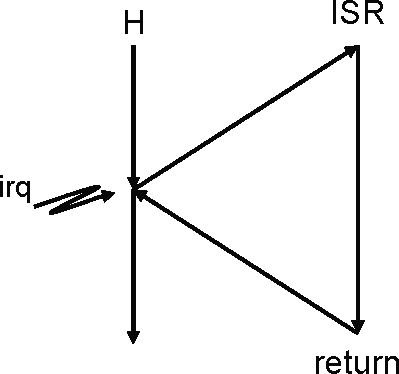
\includegraphics[scale=\figscale]{images/intsimpleinterruptdispatch}
\caption{Eenvoudige voorstelling van een interruptafhandeling.}
\label{fig:intsimpleinterruptdispatch}
\end{figure}

ISR's lijken veel op gewone subroutines, maar er zijn verschillen:

\begin{itemize}
\item Een ISR wordt gestart door een interrupt, niet door een
instructie\footnote{Er zijn processoren die instructies hebben die
software-interrupts genereren, zoals de Intel x86-familie.}.

\item Direct nadat de interrupt is herkend, wordt de Global Interrupt Enable
vlag (de I-vlag) in het Status Register op 0 gezet. Dit zorgt ervoor dat de
ISR niet kan worden onderbroken door een (nieuwe) interruptaanvraag.

\item Voor terugkeer moet de instructie \lstinline|RETI| (Return From
Interrupt) gebruikt worden. Deze instructie zet de Global Interrupt Enable
vlag weer aan.
\end{itemize}

Interrupts en subroutines hebben wel \'e\'en overeenkomst: in beide gevallen
wordt de program counter (PC) op de stack gezet. Dit wordt uitgebeeld in
figuur~\ref{fig:intinterruptdispatchwithstackandiflag}. Omdat het
terugkeeradres op de stack wordt gezet, moet de stack pointer (SP) worden
ge\"initialiseerd v\'o\'ordat de interrupts mogen worden afgehandeld. Dat
betekent dat direct naar het starten van het lopende programma, bijvoorbeeld
na een reset, de interrupts nog niet mogen worden afgehandeld omdat de
stack pointer nog niet is ge\"initialiseerd.

\begin{figure}[!ht]
\centering
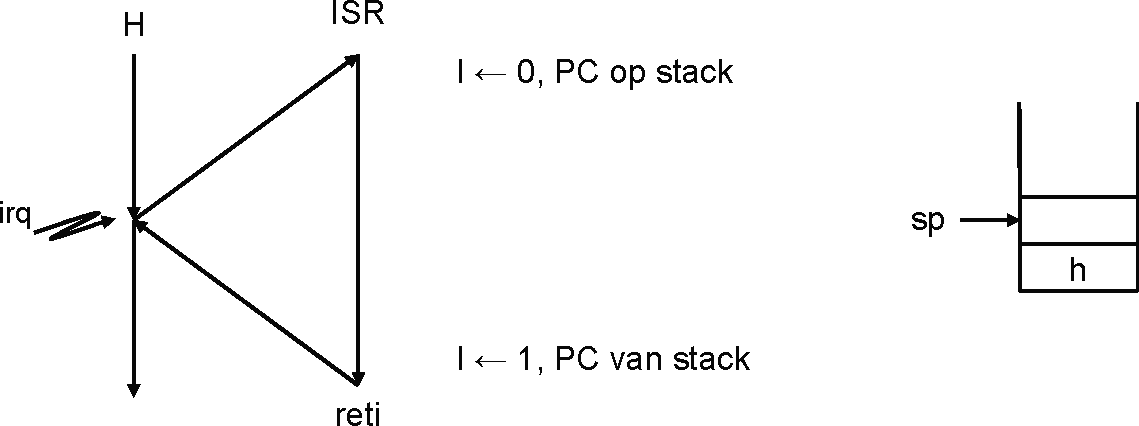
\includegraphics[scale=\figscale]{images/intinterruptdispatchwithstackandiflag}
\caption{Interruptafhandeling: de Program Counter wordt op de stack gezet.}
\label{fig:intinterruptdispatchwithstackandiflag}
\end{figure}

Twee instructies be\"invloeden direct de I-flag:

\qquad \lstinline|sei| - set Global Interrupt Enable flag, interrupts worden afgehandeld.

\qquad\lstinline|cli| - clear Global Interrupt Enable flag, interrupts worden geblokkeerd.

De I-vlag is gepositioneerd op bit 7 van het Status Register (SREG). Zie
figuur~\ref{fig:intsregregisterlayout}.

%%%% SREG
\begin{figure}[!ht]
\renewcommand\arraystretch{1.4}
%\footnotesize
\scriptsize
\centering
\begin{tabu} to 0.9\textwidth {X[,c,]X[,c,]X[,c,]X[,c,]X[,c,]X[,c,]X[,c,]X[,c,]}
7 & 6 & 5 & 4 & 3 & 2 & 1 & 0 \\
\hline
\multicolumn{1}{|c}{I} & \multicolumn{1}{|c}{T} & \multicolumn{1}{|c}{H} & \multicolumn{1}{|c}{S} & \multicolumn{1}{|c}{V} & \multicolumn{1}{|c}{N} & \multicolumn{1}{|c}{Z} & \multicolumn{1}{|c|}{C} \\ \hline
R/W & R/W & R/W & R/W & R/W & R/W & R/W & R/W \\
0 & 0 & 0 & 0 & 0 & 0 & 0 & 0 \\
\end{tabu}
\caption{Status Register SREG.}
\label{fig:intsregregisterlayout}
\end{figure}
%%%% SREG

Pas na het initialiseren van de stack pointer mag de instructie
\lstinline|sei| gegeven worden.


\section{Interruptbronnen}
De ATmega32 kent veel interruptbronnen. Zo kan de ATmega32 reageren op
drie externe interrupts: INT0, INT1 en INT2. Verder kan de analoog-digitaal
converter (ADC) een interrupt geven als de conversie klaar is. De seri\"ele
interface (USART) kent naast een interrupt wanneer een karakter is ontvangen
ook een interrupt voor wanneer een karakter is verzonden. De nog te bespreken
timer/counters (zie hoofdstuk~\ref{cha:timercounters}) kunnen een interrupt
afgeven wanneer een timer/counter ``over de kop'' gaat, dus wanneer een
timer/counter van de hoogste stand naar de laagste stand gaat. Verder zijn
er nog interrupts mogelijk van de EEPROM, de TWI- en de SPI-interface.

Al deze interruptbronnen hebben een eigen interrupt-enable-bit. Om een
interrupt van een bron ook daadwerkelijk te laten plaatsvinden, moet deze
bit geactiveerd zijn (logisch~1) \'en de I-vlag moet logisch 1 zijn.

De ATmega32 heeft geen \textsl{software interrupts}. Dat zijn
software-instructies die interrupts genereren. Deze zijn wel na te bootsen
met INT0, INT1 en INT2.


\section{De Interrupt Vector Table}
We hebben nu besproken hoe het verwerken van een interrupt wordt uitgevoerd.
Maar nu rijst de vraag: waar moet de ISR beginnen? We zouden hiervoor een
vast adres in de Flash-ROM kunnen kiezen, bijvoorbeeld adres 0x1000.
Vervolgens reserveren we 512 bytes voor de ISR. De volgende ISR begint dan
op adres 0x1200. Hoewel dit natuurlijk te realiseren is, kleven hier wel
wat bezwaren aan. Ten eerste moet de ISR altijd op adres 0x1000 beginnen.
Ten tweede kan de ISR niet groter zijn dan 512 bytes. Als de ISR korter is
dan 512 bytes, dan gebruiken we een gedeelte van de Flash-ROM niet (bedenk
dat de volgende ISR op adres 0x1200 begint). Ten derde moet de Flash-ROM
minimaal 4608 (= 0x1200) bytes groot zijn. We zien nu dat een vast adres
en een vaste lengte voor een ISR niet flexibel is.

We kunnen deze drie problemen oplossen door gebruik te maken van een
\textsl{Interrupt Vector Table}.






\begin{figure}[!ht]
\centering
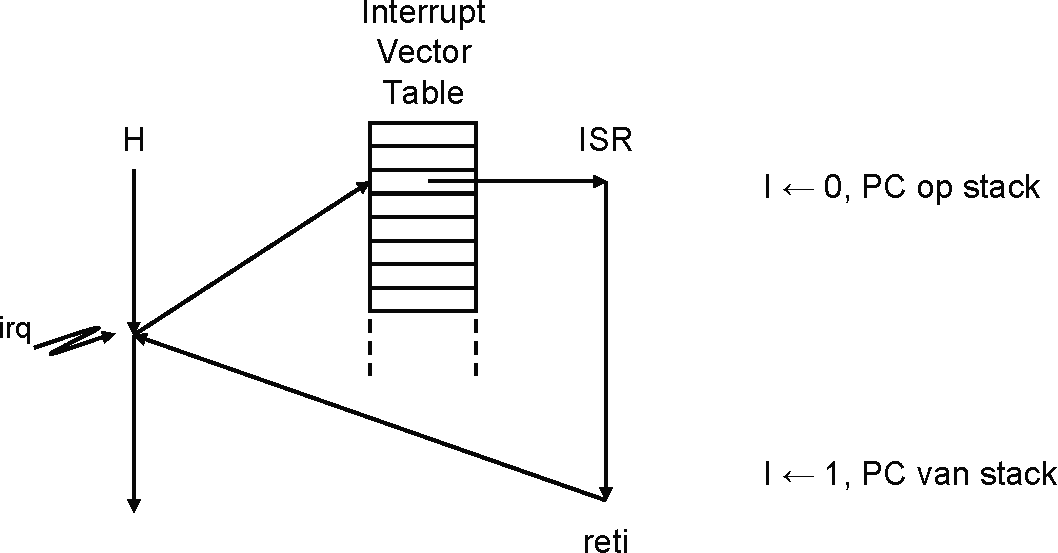
\includegraphics[scale=\figscale]{images/intinterruptdispatchwithvectortable}
\caption{Interruptafhandeling: gebruik van de Interrupt Vector Table.}
\label{fig:intinterruptdispatchwithvectortable}
\end{figure}



\section{Stappen in de interruptverwerking}
Als een interruptsignaal bij de processor binnenkomt, worden de volgende
stappen genomen:
\begin{enumerate}
\item De processor maakt de instructie af die op dat moment wordt uitgevoerd.
      Dit is een instructie in het programma.
\item De processor slaat het adres van de volgende instructie op de stack op.
      Dit adres staat in de program counter. De Global Interrupt Enable vlag
      wordt op 0 gezet.
\item De processor springt naar de \textsl{interrupt vector}. Dit is een vaste
      geheugenlocatie in de Flash-ROM.
\item Vanuit de interrupt vector wordt gesprongen naar naar het adres van de
      daadwerkelijke interrupt service routine (ISR).
\item Bij terugkeer uit de ISR wordt de program counter geladen met de adres
      dat op de stack gezet was. De Global Interrupt Enable vlag wordt op 1
      gezet.
\item De processor vervolgt het uitvoeren van het programma. Er wordt altijd
      \'e\'en instructie uitgevoerd voordat een eventuele nieuwe interrupt
      wordt verwerkt.
\end{enumerate}

\begin{table}[!ht]
\centering
\caption{Interrupt vectortabel voor de ATmeag32(A).}
\setlength{\tabcolsep}{8pt}
\begin{tabu}{ccll}
\toprule
vector \# & ROM-adres & Bron          & Omschrijving \\ \midrule
 1        & 0x000     & RESET         & Reset vector \\
 2        & 0x002     & INT0          & External Interrupt request 0 \\
 3        & 0x004     & INT1          & External Interrupt request 1 \\
 4        & 0x006     & INT2          & External Interrupt request 2 \\
 5        & 0x008     & TIMER2\_COMP  & Timer/Counter2 Compare Match \\
 6        & 0x00A     & TIMER2\_OVF   & Timer/Counter2 Overflow \\
 7        & 0x00C     & TIMER1\_CAPT  & Timer/Counter1 Capture Event \\
 8        & 0x00E     & TIMER1\_COMPA & Timer/Counter1 Compare Match A \\
 9        & 0x010     & TIMER1\_COMPB & Timer/Counter1 Compare Match B \\
10        & 0x012     & TIMER1\_OVF   & Timer/Counter1 Overflow \\
11        & 0x014     & TIMER0\_COMP  & Timer/Counter0 Compare Match \\
12        & 0x016     & TIMER0\_OVF   & Timer/Counter0 Overflow \\
13        & 0x018     & SPI, STC      & Serial Transfer Complete \\
14        & 0x01A     & USART, RXC    & USART, Rx Complete \\
15        & 0x01C     & USART, UDRE   & USART Data Register Empty \\
16        & 0x01E     & USART, TXC    & USART, Tx Complete \\
17        & 0x020     & ADC           & ADC Conversion Complete \\
18        & 0x022     & EE\_RDY       & EEPROM Ready \\
19        & 0x024     & ANA\_COMP     & Analog Comparator \\
20        & 0x026     & TWI           & Two-wire Serial Interface \\
21        & 0x028     & SPM\_RDY      & Store Program Memory Ready \\
\bottomrule
\end{tabu}
Noot: het ROM-adres is in words.
\end{table}

\section{Interruptresponstijd}
De responstijd voor alle ingeschakelde interrupts van de ATmega32 is minimaal vier klokcycli.
Tijdens deze vier klokcyclusperiode wordt de program counter op de stack geplaatst (twee bytes)
en wordt de program counter geladen met het vectoradres van de interrupt.
Na vier klokcycli wordt gesprongen naar het vectoradres van de interrupt die wordt gehonoreerd.
De instructie op de vector is normaal gesproken een sprong naar de interruptroutine en deze
sprong duurt drie klokcycli.

Als een interrupt optreedt tijdens de uitvoering van een instructie met meerdere cycli dan
wordt deze instructie voltooid voordat de interrupt wordt gehonoreerd. Staat de ATmega32 in
slaapstand dan wordt de responstijd met vier klokcycli verhoogd. Deze verhoging komt bovenop
de opstarttijd van de geselecteerde slaapmodus.

Een terugkeer (return) uit een interruptroutine duurt vier klokcycli. Tijdens deze vier
klokcycli wordt de program counter van de stack gehaald (twee bytes) en wordt de stack
pointer met twee verhoogd. Tevens word de I-bit in het statusregister op 1 gezet.

\section{Context switch}

\begin{lstlisting}[language=AVRassembler,caption=Opslaan van de vlaggen.,label=cod:contextswich]
ISR:	push r16		; push R16
		in   r16,SREG	; SREG in I/O memory ...
		push r16		; ... so push flags via R16

		pop  r16		; pop flags via R16
		out  SREG,r16
		pop  r16		; pop R16
		reti			; return
\end{lstlisting}

\section{Externe interrupts}
De General Interrupt Control Register (GICR) heeft drie bits waarmee de INT’s kunnen worden geactiveerd.

Een logische 1 in het betreffende bit activeert de INT.

De I-flag moet 1 zijn om interrupt ook daadwerkelijk te herkennen.


%%%% GICR
\begin{figure}[!ht]
\renewcommand\arraystretch{1.4}
%\footnotesize
\scriptsize
\centering
\begin{tabu} to 0.9\textwidth {X[,c,]X[,c,]X[,c,]X[,c,]X[,c,]X[,c,]X[,c,]X[,c,]}
7 & 6 & 5 & 4 & 3 & 2 & 1 & 0 \\
\hline
\multicolumn{1}{|c}{INT0} & \multicolumn{1}{|c}{INT1} & \multicolumn{1}{|c}{INT2} & \multicolumn{1}{|c}{\cellcolor{lightgrey} $-$} & \multicolumn{1}{|c}{\cellcolor{lightgrey} $-$} & \multicolumn{1}{|c}{\cellcolor{lightgrey} $-$} & \multicolumn{1}{|c}{\cellcolor{lightgrey} IVSEL} & \multicolumn{1}{|c|}{\cellcolor{lightgrey} IVCE} \\ \hline
R/W & R/W & R/W & R/W & R/W & R/W & R/W & R/W \\
0 & 0 & 0 & 0 & 0 & 0 & 0 & 0 \\
\end{tabu}
\caption{GICR register}
\label{fig:intgicr}
\end{figure}
%%%% GICR


\setcounter{chapter}{1}
%\chapter{Timer/Counter 0}
\label{cha:timercounters}
In veel applicaties moet gewacht worden, bijvoorbeeld elke seconde een meting doen,
waterklep 1 seconde open. Het meten van deze tijd (wachten) is op te lossen door
middel van de bekende wachtlus. De processor kan dan echter geen andere taken
uitvoeren en dat is in veel situaties w\'el gewenst. Denk hierbij aan Real Time
systemen en besturingssystemen. Beter is deze tijd hardwarematig te meten.
Een \textsl{timer} kan dan uitkomst bieden. Een timer is niets anders dan een teller
die op iedere klokpuls, bijvoorbeeld van de oscillator, wordt verhoogd. Na een bepaald
aantal klokpulsen heeft de timer de hoogste stand bereikt en begint weer opnieuw.
Er wordt dan een overflow-signaal afgegeven. Dit signaal genereert, indien geactiveerd,
een interrupt.

Dezelfde schakeling kan ook gebruikt worden om extern aangeboden pulsen te tellen.
Dit wordt dan een \textsl{counter} genoemd. Met de combinatie van een counter en een
timer kan een \textsl{frequentiemeter} gemaakt worden. E\'en timer meet de tijd van 1
seconde en een (andere) counter telt in die tijd het aantal aangeboden pulsen.

Timer/Counter 0 is de eerste van de drie timer/counters van de ATmega32 die
besproken worden. Het is een 8-bits timer/counter wat inhoudt dat het kan tellen
tussen 0 en~255. Als de timer/counter intern opgewekte klokpulsen telt spreken
we van een timer. Bij het tellen van extern opgewekte klokpulsen spreken
we van een counter. Technisch gezien is er geen verschil tussen de hardware
van een timer en een counter. Het verschil is dus alleen wat de klokbron is.

Timer/Counter 0 heeft vier werkmodi:
\begin{itemize}
\item Normal mode: de Timer/Counter 0 telt van 0 tot en met 255 en begint dan
weer bij 0. Zowel interne ale externe klokpulsen kunnen geteld worden.
\item CTC-mode: de Timer/Counter telt van 0 tot een van te voren opgegeven
maximale waarde en begint dan weer op 0. Zowel interne als externe klokpulsen
kunnen geteld worden.
\item Fast PWM-mode: de Timer/Counter telt van 0 tot 255 en begint dan weer op~0.
Deze modus wordt voornamelijk gebruikt om een signaalvorm op \'e\'en van de externe
pinnen van de ATmega32 te genereren.
\item Phase correct PWM-mode: de Timer/Counter telt omhoog van 0 tot en met 255
en telt dan weer omlaag tot en met 0. Deze modus wordt voornamelijk gebruikt om een
signaalvorm op \'e\'en van de externe pinnen van de ATmega32 te genereren.
\end{itemize}

In alle werkmodi is het mogelijk om een interrupts te genereren. Elke interrupt
is gekoppeld aan een eigen interruptvector.


\begin{lstlisting}[language=AVRassembler,caption=Test.]
    ldi r16,16    ; load R16 with value 16
    LDI R16,16    ; the same
\end{lstlisting}

\begin{lstlisting}[language=C,caption=Test.]
int main(void) {
    return 0;
}
\end{lstlisting}



\section{De registers van Timer/Counter 0}
De besturing van Timer/Counter 0 is vastgelegd in het TCCR0-register, zie
figuur~\ref{fig:tccr0}. Dit register kan zowel gelezen als geschreven worden.

%%%% TCCR0
\begin{figure}[!ht]
\renewcommand\arraystretch{1.4}
%\footnotesize
\scriptsize
\centering
\begin{tabu} to 0.9\textwidth {X[,c,]X[,c,]X[,c,]X[,c,]X[,c,]X[,c,]X[,c,]X[,c,]}
7 & 6 & 5 & 4 & 3 & 2 & 1 & 0 \\
\hline
\multicolumn{1}{|c}{FOC0} & \multicolumn{1}{|c}{WGM00} & \multicolumn{1}{|c}{COM01} & \multicolumn{1}{|c}{COM00} & \multicolumn{1}{|c}{WGM01} & \multicolumn{1}{|c}{CS02} & \multicolumn{1}{|c}{CS01} & \multicolumn{1}{|c|}{CS00} \\ \hline
W & R/W & R/W & R/W & R/W & R/W & R/W & R/W \\
0 & 0 & 0 & 0 & 0 & 0 & 0 & 0 \\
\end{tabu}
\caption{TCCR0 register}
\label{fig:tccr0}
\end{figure}
%%%% TCCR0

\textbf{Bit 7 -- FOC0: Force Output Compare}\\
De FOC0-bit is alleen actief als we de WGM0\textsl{x}-bits non-PWM-modus specificeren. Bij
het specificeren van \'e\'en van de twee PWM-modi moet deze bit altijd als 0 geschreven
worden. Als deze bit met een 1 geladen wordt, zal de signaalvormgenerator een directe
compare match krijgen en zal de OC0-uitgang veranderen zoals is vastgelegd in de
COM0\textsl{x}-bits.

%%%The FOC0 bit is only active when the WGM00 bit specifies a non-PWM mode. However, for
%%%ensuring compatibility with future devices, this bit must be set to zero when TCCR0 is written
%%%when operating in PWM mode. When writing a logical one to the FOC0 bit, an immediate compare
%%%match is forced on the Waveform Generation unit. The OC0 output is changed according to
%%%its COM01:0 bits setting. Note that the FOC0 bit is implemented as a strobe. Therefore it is the
%%%value present in the COM01:0 bits that determines the effect of the forced compare.

\textbf{Bits 3,6 -- WGM0\textsl{x} signaalvormgeneratorbits}\\
Deze bits bepalen de telvolgorde van de Timer/Counter, de maximale telwaarde en het type
van de signaalvormgenerator. Zie tabel~\ref{tab:signaalvormgeneratie0}.

\begin{table}[!ht]
\centering
\caption{Signaalvormgeneratie}
\label{tab:signaalvormgeneratie0}
\renewcommand\arraystretch{1.2}
\begin{tabu} {cc|l|l|l|l}
WGM01 & WGM00 & Modus & Top & Update OCR0 & TOV0-vlag \\ \hline
  0   &   0   & Normaal & 255 & direct & 255 \\
  0   &   1   & Phase Correct PWM & 255 & 255 & 0 \\
  1   &   0   & CTC & OCR0 & direct & 255 \\
  1   &   1   & Fast PWM & 255 & 0 & 255
\end{tabu}
\end{table}

\textbf{Bits 5,4 -- COM0\textsl{x} Compare Match Output Mode}\\
Deze bits bepalen het gedrag van de Output Compare pin (OC0).
Merk op dat de Data Direction (DDR) bit van de OC0-pin op 1 gezet
moet worden om de uitgang te activeren.
Tabel~\ref{tab:comparematchnonpwm0} geeft de functionaliteit van
de COM0\textsl{x}-bits weer in non-PWM-modus (Normal en CTC).

\begin{table}[!ht]
\centering
\caption{Compare Match uitgang, non-PWM-modus.}
\label{tab:comparematchnonpwm0}
\renewcommand\arraystretch{1.2}
\begin{tabu} {cc|l}
COM01 & COM00 & Beschrijving \\ \hline
  0   &   0   & Normale poortwerking, OC0 is gedeactiveerd \\
  0   &   1   & Verander OC0 op een compare match (toggle) \\
  1   &   0   & Zet OC0 op 0 op een compare match \\
  1   &   1   & Zet OC0 op 1 op een compare match \\
\end{tabu}
\end{table}

Tabel~\ref{tab:comparematchfastpwm0} geeft de functionaliteit van de
COM0\textsl{x}-bits weer in Fast PWM-modus.

\begin{table}[!ht]
\centering
\caption{Compare Match uitgang, Fast PWM-modus.}
\label{tab:comparematchfastpwm0}
\renewcommand\arraystretch{1.2}
\begin{tabu} {cc|l}
COM01 & COM00 & Beschrijving \\ \hline
  0   &   0   & Normale poortwerking, OC0 is gedeactiveerd \\
  0   &   1   & Niet gebruikt \\
  1   &   0   & Zet OC0 op 0 op een compare match, zet op 1 op TCNT = 255 \\
  1   &   1   & Zet OC0 op 1 op een compare match, zet op 0 op TCNT = 255 \\
\end{tabu}
\end{table}

Tabel~\ref{tab:comparematchphasecorrectpwm0} geeft de functionaliteit van de
COM0\textsl{x}-bits weer in Phase Correct PWM-modus.

\begin{table}[!ht]
\centering
\caption{Compare Match uitgang, Fast PWM-modus.}
\label{tab:comparematchphasecorrectpwm0}
\renewcommand\arraystretch{1.2}
\begin{tabu} {cc|p{11cm}}
COM01 & COM00 & Beschrijving \\ \hline
  0   &   0   & Normale poortwerking, OC0 is gedeactiveerd \\
  0   &   1   & Niet gebruikt \\
  1   &   0   & Zet OC0 op 0 bij Compare Match bij omhoog tellen, zet OC0 op 1 bij omlaag tellen \\
  1   &   1   & Zet OC0 op 1 bij Compare Match bij omhoog tellen, zet OC0 op 0 bij omlaag tellen \\
\end{tabu}
\end{table}





\textbf{Bits 2,1,0 -- CS0\textsl{x} klokselectiebits}\\
In tabel~\ref{tab:klokselectie0} is te zien hoe een klok geselecteerd kan worden.

\begin{table}[!ht]
\centering
\caption{Klokselectie voor Timer/Counter 0.}
\label{tab:klokselectie0}
\renewcommand\arraystretch{1.2}
%\tabulinesep=1.2mm
\begin{tabu} to 0.5\textwidth{ccc|l}
CS02 & CS01 & CS00 & operatie \\ \hline
  0  &   0  &   0  & geen werking, klok is gestopt\\
  0  &   0  &   1  & $\text{CLK}_\text{IO}/1$, geen prescaler \\
  0  &   1  &   0  & $\text{CLK}_\text{IO}/8$, van prescaler \\ 
  0  &   1  &   1  & $\text{CLK}_\text{IO}/64$, van prescaler \\
  1  &   0  &   0  & $\text{CLK}_\text{IO}/256$, van prescaler \\
  1  &   0  &   1  & $\text{CLK}_\text{IO}/1024$, van prescaler \\
  1  &   1  &   0  & externe klokbron op de T0-pin, neergaande flank \\
  1  &   1  &   1  & externe klokbron op de T0-pin, opgaande flank \\
\end{tabu}
\end{table}


Het TCNT0-register is een 8-bits register en bevat de tellerwaarde van Timer/Counter~0,
zie figuur~\ref{fig:tcnt0}. Dit register kan zowel gelezen als geschreven worden. Bij
een schrijfactie telt Timer/Counter~0 verder vanaf de geschreven waarde.

%%%% TCNT0
\begin{figure}[!ht]
\renewcommand\arraystretch{1.4}
%\footnotesize
\scriptsize
\centering
\begin{tabu} to 0.9\textwidth {X[,c,]X[,c,]X[,c,]X[,c,]X[,c,]X[,c,]X[,c,]X[,c,]}
7 & 6 & 5 & 4 & 3 & 2 & 1 & 0 \\
\hline
\multicolumn{8}{|c|}{TCNT0[7:0]}  \\ \hline
R/W & R/W & R/W & R/W & R/W & R/W & R/W & R/W \\
0 & 0 & 0 & 0 & 0 & 0 & 0 & 0 \\
\end{tabu}
\caption{TCNT0 register}
\label{fig:tcnt0}
\end{figure}
%%%% TCNT0

Het OCR0-register bevat een 8-bits waarde en wordt continue vergeleken met de waarde
in het TCNT0-register, zie figuur~\ref{fig:ocr0}. Als de twee register gelijk zijn aan
elkaar kan een interrupt gegenereerd worden of kan een golfvorm gegenereerd worden op
de OC0-uitgang.

%%%% OCR0
\begin{figure}[!ht]
\renewcommand\arraystretch{1.4}
%\footnotesize
\scriptsize
\centering
\begin{tabu} to 0.9\textwidth {X[,c,]X[,c,]X[,c,]X[,c,]X[,c,]X[,c,]X[,c,]X[,c,]}
7 & 6 & 5 & 4 & 3 & 2 & 1 & 0 \\
\hline
\multicolumn{8}{|c|}{OCR0[7:0]}  \\ \hline
R/W & R/W & R/W & R/W & R/W & R/W & R/W & R/W \\
0 & 0 & 0 & 0 & 0 & 0 & 0 & 0 \\
\end{tabu}
\caption{OCR0 register}
\label{fig:ocr0}
\end{figure}
%%%% OCR0








De indeling van het TIMSK-register is te zien in figuur~\ref{fig:timsk}. Voor Timer/Counter~0
zijn alleen de bits OCIE0 (bit 1) en TOIE0 (bit 0) van belang.

%%%% TIMSK
\begin{figure}[!ht]
\renewcommand\arraystretch{1.4}
%\footnotesize
\scriptsize
\centering
\begin{tabu} to 0.9\textwidth {X[,c,]X[,c,]X[,c,]X[,c,]X[,c,]X[,c,]X[,c,]X[,c,]}
7 & 6 & 5 & 4 & 3 & 2 & 1 & 0 \\
\hline
\multicolumn{1}{|c}{\cellcolor{lightgrey} OCIE2} & \multicolumn{1}{|c}{\cellcolor{lightgrey} TOIE2} & \multicolumn{1}{|c}{\cellcolor{lightgrey} TICIE1} & \multicolumn{1}{|c}{\cellcolor{lightgrey} OCIE1A} & \multicolumn{1}{|c}{\cellcolor{lightgrey} OCIE1B} & \multicolumn{1}{|c}{\cellcolor{lightgrey} TOIE1} & \multicolumn{1}{|c}{OCIE0} & \multicolumn{1}{|c|}{TOIE0} \\ \hline
R/W & R/W & R/W & R/W & R/W & R/W & R/W & R/W \\
0 & 0 & 0 & 0 & 0 & 0 & 0 & 0 \\
\end{tabu}
\caption{TIMSK register}
\label{fig:timsk}
\end{figure}
%%%% TIMSK

\textbf{Bit 1 -- OCIE0: Timer/Counter 0 Output Compare Match Interrupt Enable} \\
Een logische 1 in deze bit zorgt ervoor dat de compare match interrupt geactiveerd wordt.
Een interrupt wordt pas daadwerkelijk uitgevoerd als de I-bit in het statusregister ook
een logische 1 is.

\textbf{Bit 0 -- TOIE0: Timer/Counter 0 Overflow Interrupt Enable} \\
Een logische 1 in deze bit zorgt ervoot dat de overflow interrupt geactiveerd wordt.
Een interrupt wordt pas daadwerkelijk uitgevoerd als de I-bit in het statusregister ook
een logische 1 is.

De indeling van het TIFR-register is te zien in figuur~\ref{fig:tifr}. Voor Timer/Counter~0
zijn alleen de bits OCF0 (bit 1) en TOV0 (bit 0) van belang.

%%%% TIFR
\begin{figure}[!ht]
\renewcommand\arraystretch{1.4}
%\footnotesize
\scriptsize
\centering
\begin{tabu} to 0.9\textwidth {X[,c,]X[,c,]X[,c,]X[,c,]X[,c,]X[,c,]X[,c,]X[,c,]}
7 & 6 & 5 & 4 & 3 & 2 & 1 & 0 \\
\hline
\multicolumn{1}{|c}{\cellcolor{lightgrey} OCF2} & \multicolumn{1}{|c}{\cellcolor{lightgrey} TOV2} & \multicolumn{1}{|c}{\cellcolor{lightgrey} ICF1} & \multicolumn{1}{|c}{\cellcolor{lightgrey} OCF1A} & \multicolumn{1}{|c}{\cellcolor{lightgrey} OCF1B} & \multicolumn{1}{|c}{\cellcolor{lightgrey} TOV1} & \multicolumn{1}{|c}{OCF0} & \multicolumn{1}{|c|}{TOV0} \\ \hline
R/W & R/W & R/W & R/W & R/W & R/W & R/W & R/W \\
0 & 0 & 0 & 0 & 0 & 0 & 0 & 0 \\
\end{tabu}
\caption{TIFR register}
\label{fig:tifr}
\end{figure}
%%%% TIFR

\textbf{Bit 1 -- OCF0: Output Compare Flag 0} \\
Deze bit wordt op een logische 1 gezet als de waarde van het OCR0-register gelijk is aan
de waarde in het TCNT0-register (compare match). Dit gebeurt op de volgende Timer/Counter
0 klokpuls. Deze bit wordt op een logische~0 gezet
als de bijbehorende interrupt wordt uitgevoerd. Als alternatief voor het op 0 zetten
kan een 1 worden geschreven naar deze bit.

\textbf{Bit 0 -- TOV0: Timer/Counter 0 Overflow Flag} \\
Deze bit wordt op een logische 1 gezet als Timer/Counter 0 een overflow veroorzaakt. Dit
gebeurt op de volgende Timer/Counter 0 klokpuls. Deze
bit wordt op 0 gezet als de bijbehorende interrupt wordt uitgevoerd. Als alternatief voor
het op 0 zetten kan een 1 worden geschreven naar deze bit. In fasecorrect PWM-modus wordt
deze bit op 1 gezet als Timer/Counter 0 van telrichting verandert op 0.

In figuur~\ref{fig:sfior} is het SFIOR-register te zien.

%%%% SFIOR
\begin{figure}[!ht]
\renewcommand\arraystretch{1.4}
%\footnotesize
\scriptsize
\centering
\begin{tabu} to 0.9\textwidth {X[,c,]X[,c,]X[,c,]X[,c,]X[,c,]X[,c,]X[,c,]X[,c,]}
7 & 6 & 5 & 4 & 3 & 2 & 1 & 0 \\
\hline
\multicolumn{1}{|c}{\cellcolor{lightgrey} ADTS2} & \multicolumn{1}{|c}{\cellcolor{lightgrey} ADTS1} & \multicolumn{1}{|c}{\cellcolor{lightgrey} ADTS0} & \multicolumn{1}{|c}{\cellcolor{lightgrey} --} & \multicolumn{1}{|c}{\cellcolor{lightgrey} ACME} & \multicolumn{1}{|c}{\cellcolor{lightgrey} PUD} & \multicolumn{1}{|c}{\cellcolor{lightgrey}PSR2} & \multicolumn{1}{|c|}{PRS10} \\ \hline
R/W & R/W & R/W & R & R/W & R/W & R/W & R/W \\
0 & 0 & 0 & 0 & 0 & 0 & 0 & 0 \\
\end{tabu}
\caption{SFIOR register}
\label{fig:sfior}
\end{figure}
%%%% SFIOR

\textbf{Bit 0 -- PRS10: Prescaler reset Timer/Counter 1 en Timer/Counter 0}\\
Wanneer deze bit met een 1 geschreven wordt, zal de prescaler van Timer/Counter 1 en
Timer/Counter 0 worden gereset. Nadat de operatie is voltooid, wordt deze bit door de
hardware op 0 gezet. Merk op dat de prescaler door zowel Timer/Counter 1 als
Timer/Counter 0 gebruikt wordt. Het be\"invloedt de werking van beide Timer/Counters.
Deze bit leest altijd als een 0.

\endinput


\end{document}